\chapter{热机}

燃料燃烧时释放出大量的热能。要利用这些热能来做有用的功,
例如举高重物,驱动车辆,就要设法把热能转化为机械能。
热机就是把热能转化为机械能的机器。

热机是怎样把热能转化为机械能的呢?在上一章图 \ref{fig:5-6} 的实验里,
酒精燃烧时释放出的热能传递给水和水蒸气,水蒸气在膨胀时做了功,它的热能转化为软木塞的机械能。

如果把试管换成坚固的金属汽缸,
把软木塞换成跟汽缸内壁紧密接触又能在汽缸内前后移动的活塞,
我们就得到了一台最简单、最原始的热机。

热机是在十七世纪伴随着工业革命的兴起而出现的,以后又不断地得到改进和发展,
所有的热机都具有一个共同的特点:燃料燃烧释放出热能,这些热能又传递给工作物质——水蒸气或燃气;
工作物质获得热能后,膨胀做功,把一部分热能转化为机械能,同时自己的热能减少,温度降低。

现在使用的热机有很多种,我们在下面只介绍最常用的内燃机。

\section{汽油机的工作原理}\label{sec:6-1}

内燃机的基本特点是让燃料在机器的气缸内燃烧,生成高温高压的燃气,
利用这个燃气作为工作物质去推动活塞做功。内燃机的名字就是由此而来的。

\begin{wrapfigure}{r}{6.5cm}
    \centering
    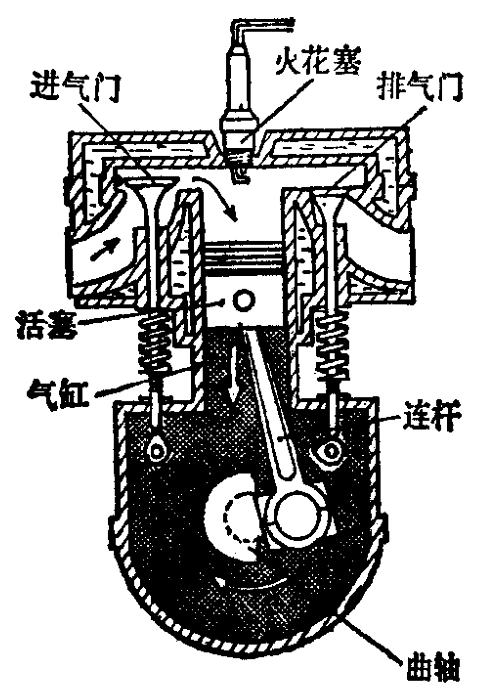
\includegraphics[width=5cm]{../pic/czwl2-ch6-1}
    \caption{}\label{fig:6-1}
\end{wrapfigure}

内燃机有两种:汽油机和柴油机。这一节,我们介绍汽油机的工作原理。

汽油机是用汽油作燃料的内燃机。它的构造如图 \ref{fig:6-1} 所示,气缸里的活塞用连杆跟曲轴相连,
气缸上面有进气门和排气门,气缸顶部有火花塞。

汽油机工作的时候,活塞在气缸里往复运动。活塞从气缸一端运动到另一端叫做一个冲程。
四冲程汽油机的工作过程是由吸气、压缩、做功、排气四个冲程组成的。

第一个冲程是吸气冲程。如 \hyperref[fig:pic3]{彩图3} 甲所示,
进气门打开,排气门关闭,活塞由最上端向下运动,气缸里气体的体积增大,压强减小(低于大气压),
于是在化油器内由汽油和空气形成的燃料混合物从进气门被吸入气缸。
当活塞到达气缸最下端的时候,进气门关闭,完成吸气冲程。

第二个冲程是压缩冲程。 如 \hyperref[fig:pic3]{彩图3} 乙所示,
进气门和排气门都关闭,活塞向上运动,燃料混合物受到压缩,压强和温度都提高了。
最后压强达到 6~15千克力/$\pflm$\footnotemark,温度升高到 250 ~ 300 ℃ 左右。
\footnotetext{千克力/$\pflm$ (即工程大气压)是工程技术上常用的压强单位,
它与帕斯卡的关系是: $1 \text{千克力/}\pflm = 9.80665 \times 10^4 \pasika$。}

第三个冲程是做功冲程。如 \hyperref[fig:pic3]{彩图3} 丙所示,
在压缩冲程末,火花塞产生电火花,燃料混合物猛烈燃烧,产生高温高压的燃气,
温度升高到 2000 ~ 2500 ℃,压达到 30 ~ 50 千克力/$\pflm$。
于是高温高压燃气推动活塞向下运动,活塞又通过连杆使曲轴转动。

第四个冲程是排气冲程。如 \hyperref[fig:pic3]{彩图3} 丁所示,
进气门关闭,排气门打开,活塞向上运动,把废气排出气缸。

排气冲程末,排气门关闭,进气门打开,活塞再向下运动,又开始了新的吸气冲程。

在汽油机工作时,上面所讲的四个冲程是周而复始循环不停的,
所以把这四个冲程叫做一个工作循环。每一个循环,活塞往复两次,曲轴转动两周。

汽油机在四个冲程中,只有做功冲程燃气对外做功;其他三个冲程是辅助冲程,
要靠安装在曲轴上的飞轮的惯性来完成。
从全局看,做功冲程固然是主要冲程,但其他三个冲程也是不可少的,
没有其他三个冲程就失去了做功冲程对外做功的条件。

汽油机在开始运转时,需要外力(人力或电动机的驱动力)先使曲轴转动起来,以后汽油机才能够自行工作。

汽油机比较轻巧,常用在汽车、飞机和小型农业机械(如插秧机、机动喷雾器)上面。


\section{柴油机的工作原理}\label{sec:6-2}

\begin{wrapfigure}[14]{r}{6.5cm}
    \centering
    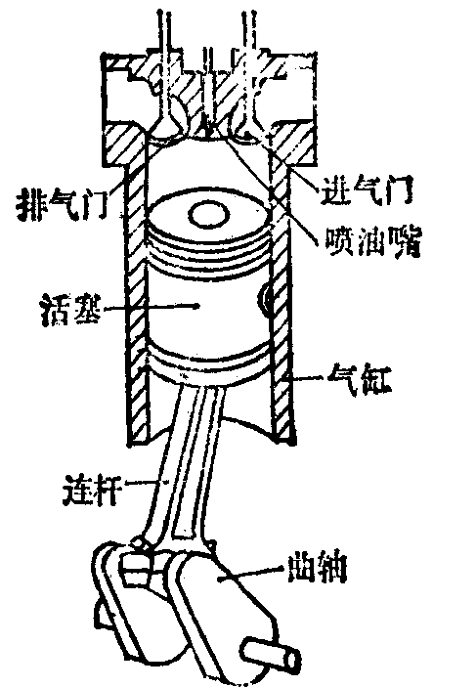
\includegraphics[width=5cm]{../pic/czwl2-ch6-2}
    \caption{柴油机}\label{fig:6-2}
\end{wrapfigure}

柴油机是用柴油作燃料的内燃机。柴油机的构造跟汽油机相似,
主要不同的是柴油机的气缸顶部有一个喷油嘴,没有火花塞(图 \ref{fig:6-2})。
柴油机的每一工作循环也是由吸气、压缩、做功和排气四个冲程组成的。
但由于使用的燃料不同,柴油机和汽油机的工作过程也有所不同。

在吸气冲程,汽油机吸入气缸里的是汽油和空气的混合物,柴油机吸入气缸里的只是空气。

\begin{enhancedline}
在压缩冲程,汽油机只把燃料混合物的体积压缩到吸气冲程末的 $\dfrac{1}{6}$ ~ $\dfrac{1}{9}$。
如果压缩得更多,在压缩过程的中途,燃料混合物就因温度升高超过燃点而燃烧,汽油机将无法正常工作。
柴油机可以把空气的体积压缩到吸气冲程末的 $\dfrac{1}{16}$ ~ $\dfrac{1}{22}$,
压强达到 35 ~ 45 千克力/$\pflm$,温度升高到 500 ~ 700 ℃ ,比汽油机里燃料混合物的压强和温度都高。
\end{enhancedline}

在做功冲程,汽油机是用火花塞点火使燃料燃烧的(这种点火方式叫做点燃式)。
柴油机是在压缩冲程末,由喷油嘴向气缸内喷射雾状柴油,
雾状柴油遇到远远超过它的燃点的热空气立即燃烧(这种点火方式叫做压燃式)。
燃气的温度达到 1700 ~ 2000 ℃ ,压强达到 50 ~ 100 千克力/$\pflm$。
在柴油机里,推动活塞做功的燃气的压强比汽油机里的高,燃气做的功较多,所以效率较高。

在排气冲程,柴油机和汽油机一样,将废气排出气缸。

柴油比汽油便宜,所以柴油机比汽油机经济,但是比较笨重,主要应用在拖拉机、坦克、轮船、内燃机车、载重汽车上。
在没有电源的地方,常用它带动水泵和各种农业加工机械工作,或带动发电机发电。


\section{热机的效率}\label{sec:6-3}

跟所有的机器一样,热机也有一个效率问题。
任何热机都不可能把燃料释放的热能全部用来做有用功。
废气要带走一部分热能,热机部件散热要损失一些热能,
另外,克服机件之间的摩擦做功,也要消耗一部分能量。

\CJKunderwave{在热机里,用来做有用功的那部分能量跟燃料完全燃烧所放出的能量之比,叫做热机的效率}。
热机的效率通常用百分数来表示,汽油机的效率是 20 ~ 30\%,柴油机的效率是 28 ~ 40 \% 。

热机的效率是热机性能的重要标志之一,如何提高热机的效率是减少能源消耗的重要问题。
要提高热机的效率,就要尽量减少各种热损失,并且要保证良好的润滑,减少因克服摩擦而额外消耗的功。


\section{热机和环境保护}\label{sec:6-4}

热机的广泛应用,促进了社会生产的发展和人们生活水平的提高。
但是,任何事物都有两面性,热机的大量应用,也会污染环境,给人们带来危害。

热机工作时往往产生很大的噪声。
火车的轰隆声,城市中大量汽车产生的噪声,干扰了人们的正常工作和生活。
热机工作都要消耗燃料,燃料燃烧过程中,会排出二氧化硫、氮氧化合物、一氧化碳、
二氧化碳以及飞灰等物质。这些物质对人体的健康有害。

环境污染问题,在一些工业发达的国家里,在五十年代就成了社会公害。
目前,世界各国对控制污染、保护环境都十分重视,在这方面进行了大量的研究工作,
并采取了许多保护环境的措施。

随着工业建设的发展,我国也出现了环境污染问题。
党和政府对保护环境和人民健康十分关心,已经建立了专门机构,研究解决这些问题。
我们要做到:既要发展生产,又要保护好祖国的壮丽河山,使人民有一个清洁美好的生活环境。




\section*{阅读材料:热机的发展}

\begin{wrapfigure}{r}{7cm}
    \centering
    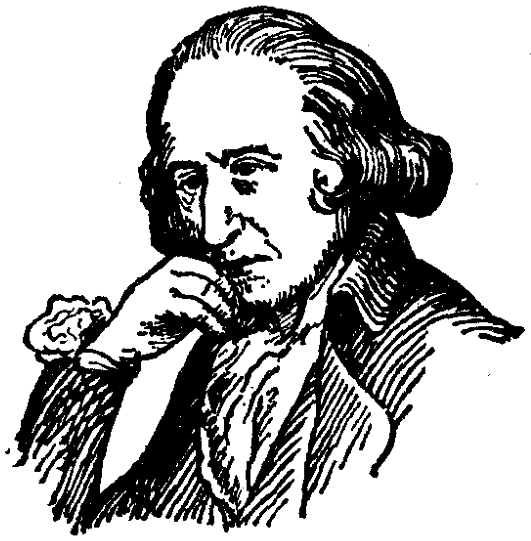
\includegraphics[width=6cm]{../pic/czwl2-ch6-watt}
    \caption*{瓦特(1736 ~ 1819)}\label{fig:6-watt}
\end{wrapfigure}

十七世纪以前,人们的生产活动除了用人力、畜力外,只能利用风力、水力来带动一些简单机械。
从十七世纪起,随着生产的发展,特别是纺织机等的陆续出现,人力、畜力、风力、水力不能满足需要了。
同时,机器制造业已经产生,使发明、制造新的动力机成为可能。

世界上最早的热机——蒸汽机就是在这种情况下发明的。
蒸汽机先后经过许多人的研究、试制和改进,其中贡献最大的是英国的工人出身的技师瓦特。
1782 年,他发明了往复式蒸汽机,使蒸汽机逐步成为一种广泛应用的动力机。

% \begin{figure}[htbp]
%     \centering
%     \begin{minipage}{4cm}
%     \centering
%     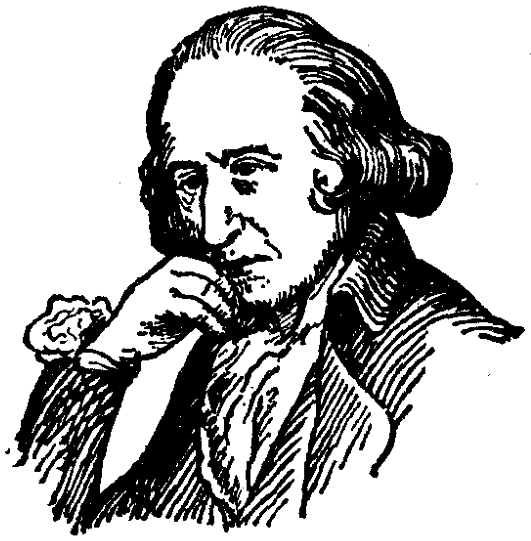
\includegraphics[width=4cm]{../pic/czwl2-ch6-watt}
%     \caption*{瓦特(1736 ~ 1819)}\label{fig:6-watt}
%     \end{minipage}
%     \qquad
%     \begin{minipage}{10cm}
%     \centering
%     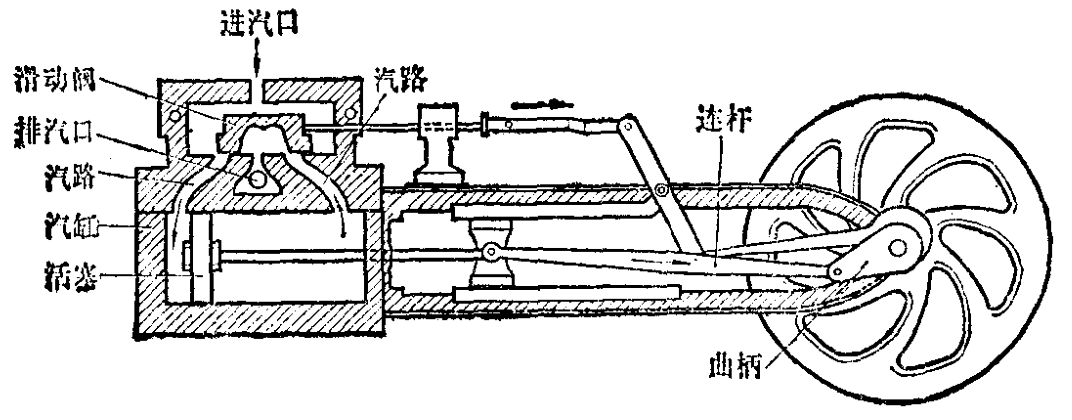
\includegraphics[width=10cm]{../pic/czwl2-ch6-3}
%     \caption{往复式蒸汽机示意图}\label{fig:6-3}
%     \end{minipage}
% \end{figure}

图 \ref{fig:6-3} 是往复式蒸汽机的示意图。
由锅炉来的
高温高压蒸汽进入汽缸  左侧,推动活塞向右运动。活塞右侧的废汽经右侧的汽路从排汽口排出。
当活塞运动到右端时,滑动阀遮住左侧的汽路,
高温高压蒸汽进入汽缸的右侧,推动活塞向左运动,活塞左侧的废汽经左侧的汽路从排汽口排出。
这样,蒸汽使活塞不停地做往复运动。活塞的往复运动,通过连杆、曲柄,使机轴和飞轮转动。

\begin{figure}[htbp]
    \centering
    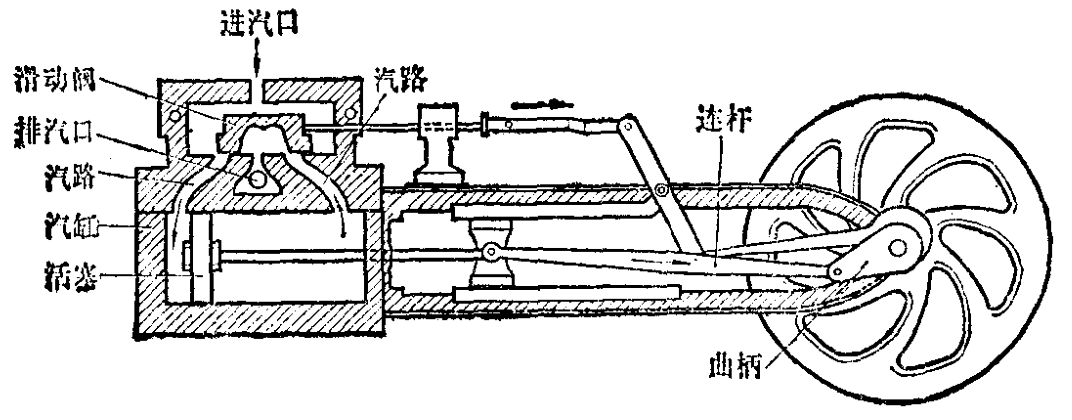
\includegraphics[width=0.8\textwidth]{../pic/czwl2-ch6-3}
    \caption{往复式蒸汽机示意图}\label{fig:6-3}
\end{figure}

蒸汽机的发明对当时工业发展起了巨大的作用。
但是,蒸汽机需要庞大的锅炉生产水蒸气,还需要曲柄连杆机构把往复运动变为转动,
这就使蒸汽机十分笨重,而且效率很低,只有 6 ~ 15 \% 。
为了克服这些缺点,人们发明了不要锅炉设备的内燃机和不要曲柄连杆机构的蒸汽轮机。

属于内燃机的汽油机是在 1876 年发明的,柴油机是在 1892 年发明的。
内燃机体积小,使用起来比蒸汽机方便多了。
内燃机发明后,汽车、飞机出现了,用在农业上的拖拉机也出现了。
内燃机的广泛应用,对生产技术的发展起了很大的促进作用。

蒸汽轮机是 1884 年出现的,它的基本特点是让锅炉里来的高温高压蒸汽从喷嘴高速喷出,
冲击叶轮的叶片,直接使机轴转动(图 \ref{fig:6-4})。
蒸汽轮机的效率比蒸汽机高得多,一般是 25 ~ 30 \%。
目前大型火力发电站大多采用蒸汽轮机。现代的蒸汽轮机的功率达到几十万千瓦。

\begin{wrapfigure}{r}{7cm}
    \centering
    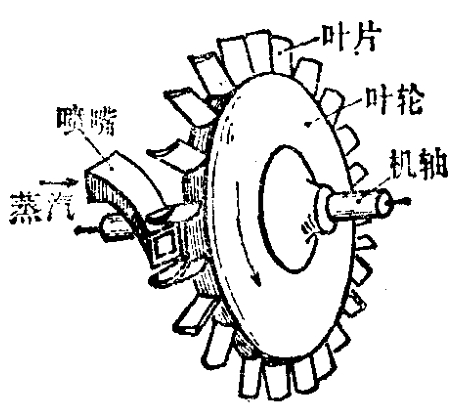
\includegraphics[width=6cm]{../pic/czwl2-ch6-4}
    \caption{}\label{fig:6-4}
\end{wrapfigure}

最近几十年来,人们吸取内燃机和蒸汽轮机的特点,研制成了燃气轮机。
它是让高温高压的燃气直接冲击叶轮的叶片而做功的,它没有笨重的锅炉设备,也不用曲柄连杆机构。
因此,燃气轮机的体积小、重量轻、效率高(可以达到 50 ~ 60 \% )。
但是,燃气轮机让高温高压的燃气直接冲击叶片,这就要求使用性能优良的耐热材料来制造叶片,
而且要有很好的冷却设备,以保证机器在工作中不致过热。
燃气轮机首先应用在飞机上,目前在火车和火力发电站上也已开始试用。

现代喷气式飞机上应用的发动机是一种新型的热机——空气喷气发动机。
喷气发动机是让高温高压的燃气高速地向后喷出,而使发动机获得向前的动力。
空气喷气发动机需要利用空气中的氧气来帮助燃料燃烧,因此,
使用这种热机的飞行器不能飞到大气层以外的空间里去。
另外还有一种喷气发动机,它既带燃料,又带氧化剂,不需要空气中的氧气助燃。
这种发动机就是火箭喷气发动机,常简称火箭。
火箭是人类征服宇宙空间的工具,人造地球卫星就是用火箭发射的。

从蒸汽机出现以来,热机已经发展到了很高的水平。
但是事物总是不断发展的,随着科学技术水平的提高,必定会有更好、更新的热机出现,为人们的生产和生活带来更多的方便。


\section*{复习题}

(1) 热机的共同特点是什么?

(2) 简述四冲程汽油机的工作过程,并分析压缩冲程和做功冲程中能的转化。

(3) 汽油机和柴油机的工作过程有什么不同?

(4) 什么叫热机的效率?



